\let\negmedspace\undefined
\let\negthickspace\undefined
\documentclass[journal]{IEEEtran}
\usepackage[a5paper, margin=10mm, onecolumn]{geometry}
%\usepackage{lmodern} % Ensure lmodern is loaded for pdflatex
\usepackage{tfrupee} % Include tfrupee package

\setlength{\headheight}{1cm} % Set the height of the header box
\setlength{\headsep}{0mm}     % Set the distance between the header box and the top of the text

\usepackage{gvv-book}
\usepackage{gvv}
\usepackage{cite}
\usepackage{amsmath,amssymb,amsfonts,amsthm}
\usepackage{algorithmic}
\usepackage{graphicx}
\usepackage{textcomp}
\usepackage{xcolor}
\usepackage{txfonts}
\usepackage{listings}
\usepackage{enumitem}
\usepackage{mathtools}
\usepackage{gensymb}
\usepackage{comment}
\usepackage[breaklinks=true]{hyperref}
\usepackage{tkz-euclide} 
\usepackage{listings}
% \usepackage{gvv}                                        
\def\inputGnumericTable{}                                 
\usepackage[latin1]{inputenc}                                
\usepackage{color}                                            
\usepackage{array}                                            
\usepackage{longtable}                                       
\usepackage{calc}                                             
\usepackage{multirow}                                         
\usepackage{hhline}                                           
\usepackage{ifthen}                                           
\usepackage{lscape}
\usepackage{multicol}
\begin{document}

\bibliographystyle{IEEEtran}
\vspace{3cm}

\title{1.1.12}
\author{EE25BTECH11012-BEERAM MADHURI}
% \maketitle
% \newpage
% \bigskip
{\let\newpage\relax\maketitle}

\renewcommand{\thefigure}{\theenumi}
\renewcommand{\thetable}{\theenumi}
\setlength{\intextsep}{10pt} % Space between text and floats


\numberwithin{equation}{enumi}
\numberwithin{figure}{enumi}
\renewcommand{\thetable}{\theenumi}


\textbf{Question}:\\
 Given closed-loop transfer function $T(s) = \frac{s-5}{(s+2)(s+3)}$, the system is: \hfill (EC 2007)

\begin{enumerate}
    \item[a)] Unstable
    \item[b)] Uncontrollable
    \item[c)] Minimum phase
    \item[d)] Non-minimum phase
\end{enumerate}

\textbf{Solution:}\\
Given the closed-loop transfer function:
\begin{align}
    T(s) = \frac{s - 5}{(s + 2)(s + 3)}
\end{align}
Identifiying Poles and Zeros\\
\textbf{Poles:}\\
Set the denominator to zero: \\
\begin{align}
    (s + 2)(s + 3) = 0\\
    s = -2 ,-3
\end{align}
 Both are in the Left Half Plane (LHP).\\
\textbf{Zeros:}\\
Set the numerator to zero: 
\begin{align}
    s - 5 = 0\\
    s = +5
\end{align}
This is in the Right Half Plane (RHP).\\

Given Options:\\
a) Unstable:\\
A system is unstable if any of its poles lie in the Right Half Plane (RHP) or if there are repeated poles on the imaginary axis. (Our system is stable because poles are at -2 and -3).\\
b)Uncontrollable:\\
A property related to State-Space analysis. In transfer functions, it usually implies a pole-zero cancellation. Since no terms cancel out here, we cannot assume it is uncontrollable from this form.\\
c)Minimum Phase:\\
A system where all poles and all zeros lie in the Left Half Plane (LHP). These systems have the minimum possible phase shift for a given magnitude response.\\
d)Non-minimum Phase:\\
A system that has at least one zero (or pole) in the Right Half Plane (RHP). These systems exhibit "undershoot" in their step response and have more phase lag than a minimum phase system.\\

Determining the System Property:
Since we have a zero at $s = 5$, the system is non-minimum phase.\\
Correct Option: d) Non-minimum phase

\begin{figure}[H]
\centering
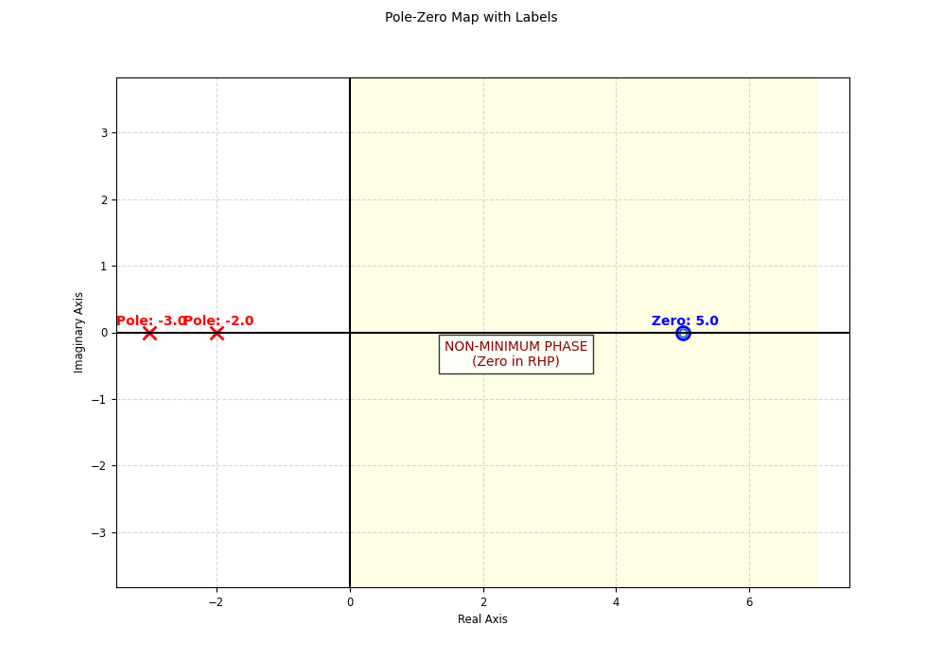
\includegraphics[width=0.85\columnwidth]{figures/plot.png}
\caption{Poles and Zeroes}
\label{fig:placeholder}
\end{figure}
\end{document}
